\documentclass[border=10pt]{standalone}

\usepackage{tikz}
\usepackage{tikzsymbols}
\usetikzlibrary{calc,patterns,shapes.geometric}

\def\centerarc[#1](#2)(#3:#4:#5){\draw[#1] ($(#2)+({#5*cos(#3)},{#5*sin(#3)})$) arc (#3:#4:#5);}

\begin{document}
	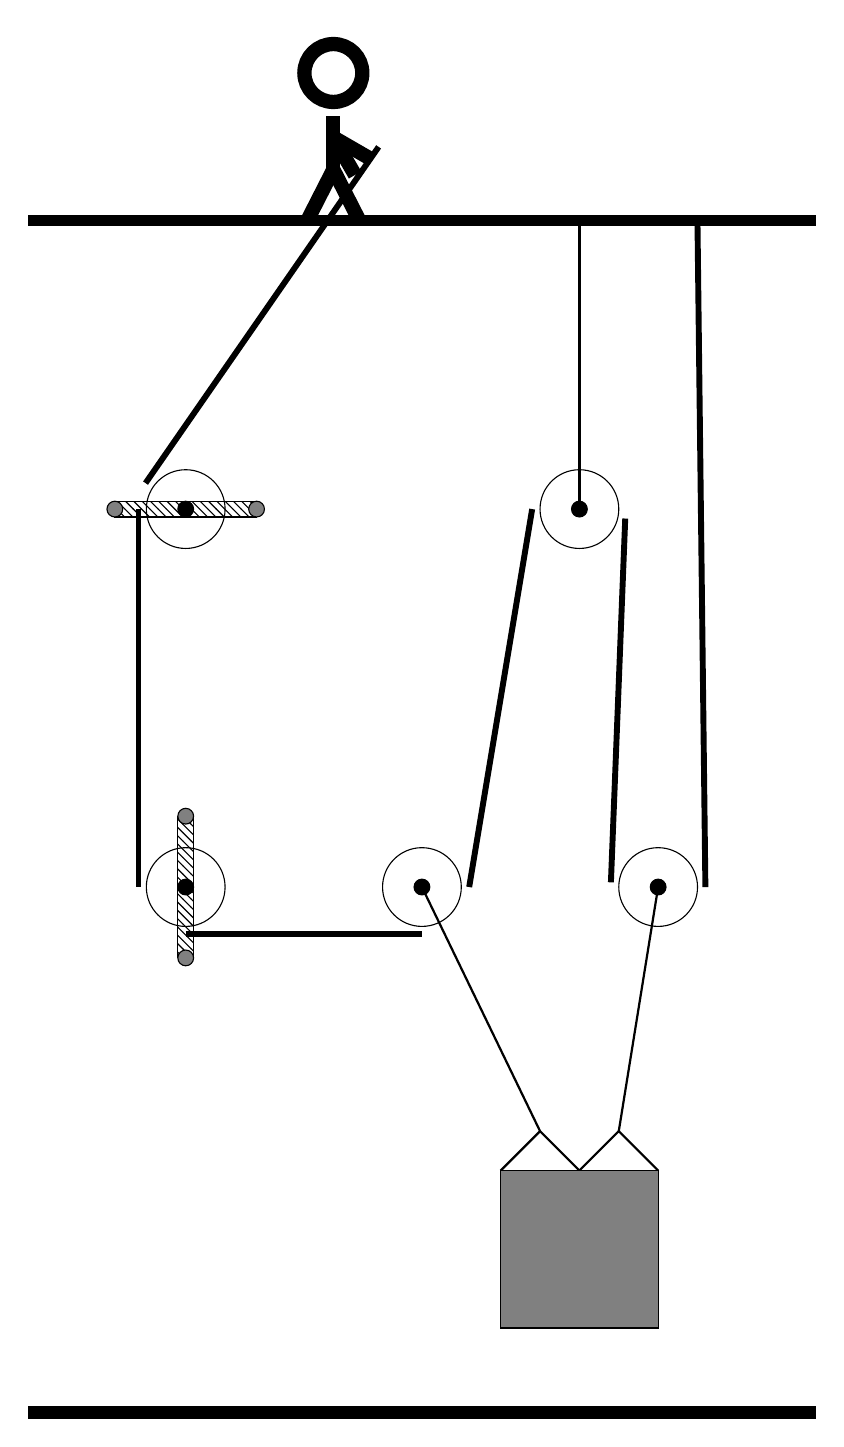
\begin{tikzpicture}
		%%%%% START %%%%%
		\draw[fill=black] (-4, 12) rectangle (6, 12.125);
		
		\draw (1, 3.6) circle (0.5);
		\draw[fill=black] (1, 3.6) circle (0.1);
		
		\draw (3, 8.4) circle (0.5);
		\draw[fill=black] (3, 8.4) circle (0.1);
		\draw[thick] (3, 8.4) -- (3, 12);
		
		\draw (4, 3.6) circle (0.5);
		\draw[fill=black] (4, 3.6) circle (0.1);
		
		\draw[thick] (4, 3.6) -- (3.5, 0.5);
		\draw[thick] (1, 3.6) -- (2.5, 0.5);
		\draw[thick]  (2, 0) -- (2.5, 0.5) -- (3, 0);
		\draw[thick]  (3, 0) -- (3.5, 0.5) -- (4, 0);
		\draw[fill=black!50] (2, 0) rectangle (4, -2);
		
		\draw (-2, 3.6) circle (0.5);
		\draw[fill=black] (-2, 3.6) circle (0.1);
		\draw[pattern=north west lines, pattern color=black] (-2.1, 4.5) rectangle (-1.9, 2.7);
		\draw[fill=black!50] (-2, 4.5) circle (0.1);
		\draw[fill=black!50] (-2, 2.7) circle (0.1);
		
		\draw (-2, 8.4) circle (0.5);
		\draw[fill=black] (-2, 8.4) circle (0.1);
		\draw[pattern=north west lines, pattern color=black] (-2.9, 8.5) rectangle (-1.1, 8.3);
		\draw[fill=black!50] (-2.9, 8.4) circle (0.1);
		\draw[fill=black!50] (-1.1, 8.4) circle (0.1);
		
		\draw[line width=0.75mm] (0.45, 13) -- (-2.51, 8.73);
		\centerarc[line width=0.75mm](-2, 8.4)(135:180:0.6);
		\draw[line width=0.75mm] (-2.6, 8.4) -- (-2.6, 3.6);
		\centerarc[line width=0.75mm](-2, 3.6)(180:270:0.6);
		\draw[line width=0.75mm](-2, 3.0) -- (1, 3.0);
		\centerarc[line width=0.75mm](1, 3.6)(270:360:0.6);
		\draw[line width=0.75mm] (1.6, 3.6) -- (2.4, 8.4);
		\centerarc[line width=0.75mm](3, 8.4)(-20:180:0.6);
		\draw[line width=0.75mm](3.582, 8.28) -- (3.4, 3.66);
		\centerarc[line width=0.75mm](4, 3.6)(160:360:0.6);
		\draw[line width=0.75mm](4.6, 3.6) -- (4.5, 12);
		
		\node at (-0.07, 13.2) {\Strichmaxerl[10][120][-30]};
		
		\draw[fill=black] (-4, -3) rectangle (6, -3.15);
		%%%%% END %%%%%
	\end{tikzpicture}
\end{document}